\documentclass[]{elsarticle} %review=doublespace preprint=single 5p=2 column
%%% Begin My package additions %%%%%%%%%%%%%%%%%%%
\usepackage[hyphens]{url}
\usepackage{lineno} % add
\providecommand{\tightlist}{%
  \setlength{\itemsep}{0pt}\setlength{\parskip}{0pt}}

\bibliographystyle{elsarticle-harv}
\biboptions{sort&compress} % For natbib
\usepackage{graphicx}
\usepackage{booktabs} % book-quality tables
%% Redefines the elsarticle footer
%\makeatletter
%\def\ps@pprintTitle{%
% \let\@oddhead\@empty
% \let\@evenhead\@empty
% \def\@oddfoot{\it \hfill\today}%
% \let\@evenfoot\@oddfoot}
%\makeatother

% A modified page layout
\textwidth 6.75in
\oddsidemargin -0.15in
\evensidemargin -0.15in
\textheight 9in
\topmargin -0.5in
%%%%%%%%%%%%%%%% end my additions to header

\usepackage[T1]{fontenc}
\usepackage{lmodern}
\usepackage{amssymb,amsmath}
\usepackage{ifxetex,ifluatex}
\usepackage{fixltx2e} % provides \textsubscript
% use upquote if available, for straight quotes in verbatim environments
\IfFileExists{upquote.sty}{\usepackage{upquote}}{}
\ifnum 0\ifxetex 1\fi\ifluatex 1\fi=0 % if pdftex
  \usepackage[utf8]{inputenc}
\else % if luatex or xelatex
  \usepackage{fontspec}
  \ifxetex
    \usepackage{xltxtra,xunicode}
  \fi
  \defaultfontfeatures{Mapping=tex-text,Scale=MatchLowercase}
  \newcommand{\euro}{€}
\fi
% use microtype if available
\IfFileExists{microtype.sty}{\usepackage{microtype}}{}
\usepackage{longtable}
\usepackage{graphicx}
% We will generate all images so they have a width \maxwidth. This means
% that they will get their normal width if they fit onto the page, but
% are scaled down if they would overflow the margins.
\makeatletter
\def\maxwidth{\ifdim\Gin@nat@width>\linewidth\linewidth
\else\Gin@nat@width\fi}
\makeatother
\let\Oldincludegraphics\includegraphics
\renewcommand{\includegraphics}[1]{\Oldincludegraphics[width=\maxwidth]{#1}}
\ifxetex
  \usepackage[setpagesize=false, % page size defined by xetex
              unicode=false, % unicode breaks when used with xetex
              xetex]{hyperref}
\else
  \usepackage[unicode=true]{hyperref}
\fi
\hypersetup{breaklinks=true,
            bookmarks=true,
            pdfauthor={},
            pdftitle={Exploratory Network Analysis of Clinical Interactions in the ED},
            colorlinks=true,
            urlcolor=blue,
            linkcolor=magenta,
            pdfborder={0 0 0}}
\urlstyle{same}  % don't use monospace font for urls
\setlength{\parindent}{0pt}
\setlength{\parskip}{6pt plus 2pt minus 1pt}
\setlength{\emergencystretch}{3em}  % prevent overfull lines
\setcounter{secnumdepth}{0}
% Pandoc toggle for numbering sections (defaults to be off)
\setcounter{secnumdepth}{0}
% Pandoc header


\usepackage[nomarkers]{endfloat}

\begin{document}
\begin{frontmatter}

  \title{Exploratory Network Analysis of Clinical Interactions in the ED}
    \author[Emory University]{Tommy Flynn\corref{c1}}
   \ead{tjflynn@emory.edu} 
   \cortext[c1]{Corresponding Author}
      \address[Emory University]{Repository
(\url{https://github.com/tommyflynn/Flynn_N741_Project/tree/master/Flynn_Project})}
  
  \begin{abstract}
  Patient acuity in the Emergency Department is triaged at the beginning
  of the care process using the Emergency Severity Index (ESI) metric. The
  ESI is presumed to predict resource consumption in the ED, and is a
  validated predictor of hospital admission for the majority of ED
  patients. It is not sensitive to non-medical patient characteristics,
  such as patient race, nor is it accountable to changes in patient
  condition over time. ED administrators and charge nurses are left with
  an impression of the unit that does not reveal the reality of current
  paitient conditions or ED resources being utilized. The lack of
  real-time ED resource and patient condition information creates
  opportunities for unrecognized patient deterioration, medical errors,
  increased wait times, and decreased patient satisfaction. An objective
  measurement of patient resource consumption that passively observes and
  calulates relative patient need in real-time would allow charge nurses
  and administrators to make informed decisions for effective, efficient,
  and safe patient care. This study tests a novel approach to measuring
  patient acuity (ED resource consumption) using real-time location system
  (RTLS) contact data and network analysis. This paper presents the
  approach and analytic results of several ED contact networks in relation
  to patient acuity (ESI)
  \end{abstract}
  
 \end{frontmatter}

\section{Research Question \& Specific
Aims}\label{research-question-specific-aims}

\begin{itemize}
\tightlist
\item
  Can network analysis of clinical interactions between patients and
  staff provide insight into the complex Emergency Department patient
  care process? (Canto et al. 2000) Aim 1: Graph the network of clinical
  interactions in the ED between patients and staff to explore potential
  similarities, future research questions, and more robust applicationg
  of igraph in R studio.
\end{itemize}

\section{Background \& Objectives}\label{background-objectives}

Intelligent clinical monitoring software is not a new idea, but
advancements in the field of data science continue to yield powerful new
tools that may make such software a reality in the near future.(Yu et
al. 2015, Donoho (2017)) Real-time location systems (RTLS) are
increasingly common in hospitals across the nation, especially in
clinical areas where patient care and flow are both complex and
time-sensitive, such as the Emergency Department (ED).(Yao, Chu, and Li
2012) A bird's-eye view of a busy urban ED might resemble a hive of
frenzied bees, but as we have learned of beehives, patterns of work and
interactions within EDs are necessarily purposed and complexly adaptive
to the various needs of the system (or hive) as a whole.(Kridi,
Carvalho, and Gomes 2016) By leveraging the technology of RTLS and
analytical power of netowrk analysis, future ED monitoring systems will
provide ED leadership with real-time resource allocation and patient
condition information. The Emergency Severity Index (ESI) is a validated
metric used to triage patients in US Emergency Departments.(Tanabe et
al. 2004) That triage nurse may decide to involve the charge nurse or a
physician given various concerns about the patient. These interactions,
observed and measured by the Real Time Location System (RTLS), continue
as more patients are triaged, moved into patient rooms, and so on toward
a vast and complex network of interactions. This web of care is likely
to correlate with the amount and quality of care delivered to individual
patients. - \textbf{The purpose of this study is to explore the network
of clinical interactions that take place in the Emergency Department and
present graphical representations of those networks.} To meet this
purpose, I received permission to analyse existing data that includes
the following; the frequency and duration of all face-to-face
interactions (patients, providers, nurses, technicians, \&
administrators) that occured in the ED for 81 12hr shifts, the location
of those interactions, and individual patients' medical and demographic
characteristics including acuity, chief complaint, gender, age, arrival
mode, and disposition. The network structural characteristics will be
assessed in relation to the industry standard acuity measure, the
Emergency Severity Index (ESI), and potential confounding variables.
Using this data will require specific knowledge of the R statistical
packages, network analysis, and data science. See Tables 1-4 for my
learning goals with respective action items, timeline, and outcomes.

\section{Methods}\label{methods}

\section{RTLS Data}\label{rtls-data}

This study applies a secondary data analysis design due to the
exploritory nature of the research aims. Data was made available with
permissions from the originating research team. The purpose of the
original study was to describe contact characteristics between patients
and staff in the ED of a busy urban hospital to inform cross-infection
control measures. Data were collected using a radio-frequency
identification system that triangulated patient and staff (nurses,
providers, and ancillary staff) locations within the ED at Emory
University Hospital Midtwon. Data for this secondary analysis were
collected using a prospective, longitudinal, observational design with a
random sampling of one day shift and one night shift per week for one
year, July 1, 2009 to June 30, 2010. This strategy was chosen to
minimize sampling bias related to seasonal or weekly fluctuations in
census, acuity, and ED staffing changes. Although a total of 104 shifts
were observed, the original research team retained only 81 shifts for
reasons related to issues with the RFID system and study staff sick
leave.(Lowery-North et al. 2013)

\section{Analysis Plan}\label{analysis-plan}

\section{Data Exploration \& Cleaning}\label{data-exploration-cleaning}

Code for analyses were maintained in private repositories in the GitHub
version control platform. Patient characteristic data was evaluated for
missing or implausible data with discriptive analyses, and RFID
generated networks will be included for statistical analysis if
variables of network density, centrality, and a network diversity scale
are distributed normally across networks. The data were inconsitant in
the way individual participants were tagged. There were 1102 unique
nodes in the vertices data, 1023 unique nodes in the edges dataset, and
1017 unique patients in the patient characteristics dataset.
Furthermore, there were a number of extra dates of data collection in
the nodes and patients data. After learning several new tricks, the data
were finally subsetted into 35 data frames to be graphed with
iGraph.(Csardi and Nepusz 2006)

\subsection{Analysis}\label{analysis}

The open-source R statistical language and R-Studio user interface from
the developers at CRAN were used for all data exploration, wrangling,
cleaning, description, and analysis.(R Core Team 2017) Pandoc's Markdown
allows for seemless integration of code, results, visualizations, and
author interpretation of the research into a single document.(Allaire et
al. 2017) Running all code and calculating all results within the
menuscript itself, Markdown eliminates risk for errors in transferring
statistical software output into foreign documents. The data were
explored, cleaned, and assessed for statistical assumptions using the
Tidyverse group of R packages.(Wickham 2017, Wickham (2016)) Data were
prepared for network visualization and plotted with the network object
package iGraph. (Csardi and Nepusz 2006).

\section{Results}\label{results}

\begin{longtable}[]{@{}cccccc@{}}
\caption{Overall Participation}\tabularnewline
\toprule
Participants (n) & Shifts & Participants/Shift & Participation Rate
(mean\%) & Total Ties & Ties/Shift\tabularnewline
\midrule
\endfirsthead
\toprule
Participants (n) & Shifts & Participants/Shift & Participation Rate
(mean\%) & Total Ties & Ties/Shift\tabularnewline
\midrule
\endhead
3635 & 35 & 103.8571 & 63.09335 & 21600 & 617.1429\tabularnewline
\bottomrule
\end{longtable}

\begin{longtable}[]{@{}ll@{}}
\caption{Patient Acuity}\tabularnewline
\toprule
Acuity Level & Count\tabularnewline
\midrule
\endfirsthead
\toprule
Acuity Level & Count\tabularnewline
\midrule
\endhead
Immediate (1) & 14\tabularnewline
Emergent (2) & 694\tabularnewline
Urgent (3) & 1191\tabularnewline
Stable (4) & 417\tabularnewline
Non Urgent (5) & 27\tabularnewline
\bottomrule
\end{longtable}

The bulk of this project ended up focussing on data exploration and
wrangling. Although the data came in tables that had been
\emph{cleaned}, there turned out to be a significant amount of wrangling
and organizing to re-clean it for the purposes of this study.

We selected 3 representative shifts for visualization and exploration.
Although I was not able to analyze these networks to the extent I had
hoped, there are a number of visualizations shown below. The first shift
represented below shows an interesting cluster of highly acute (gray)
patients, indicating that there may be something to the hypothesis that
acuity will correlate to network position.
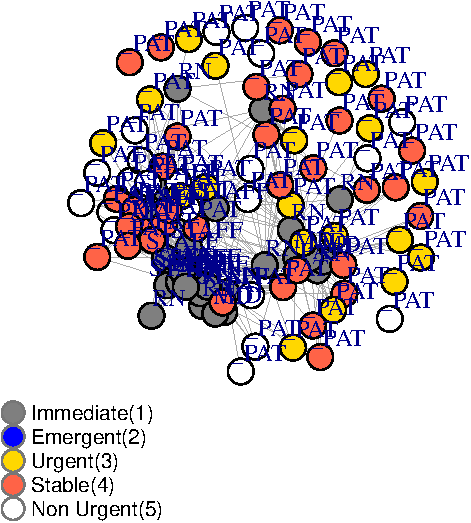
\includegraphics{Flynn_Project_files/figure-latex/shift 10-1.pdf}

The graph below is does not display the individual patient acuities, but
it does give a slightly better overview of the various positions of
patients, staff, RNs, \& MDs thoughout the network.

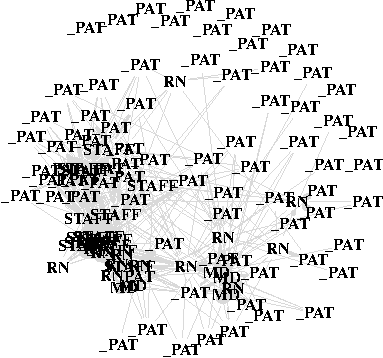
\includegraphics{Flynn_Project_files/figure-latex/shift10 labels-1.pdf}

The following network offers a unique perspective of the distribution of
ties in the network by essentially \emph{getting the nodes out of the
way}. What is particularly interesting is teh way the ties appear to be
more dense where patients are scored at an acuity of level 1, or
``Immediate''. A closer look at the distribution of edges may provide
further insights in following analyses.
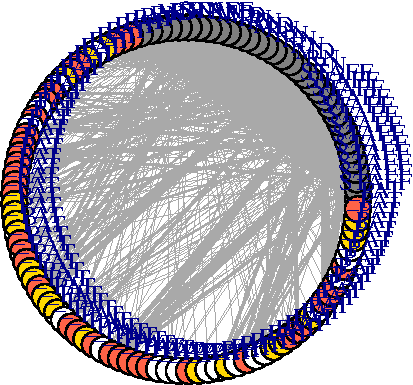
\includegraphics{Flynn_Project_files/figure-latex/shift10 circle-1.pdf}

The remaining graphs are generated from two other shifts. Although much
of the overall visual characteristics appear similar, there are a number
of interesting differences that have given me ideas for further inquiry.
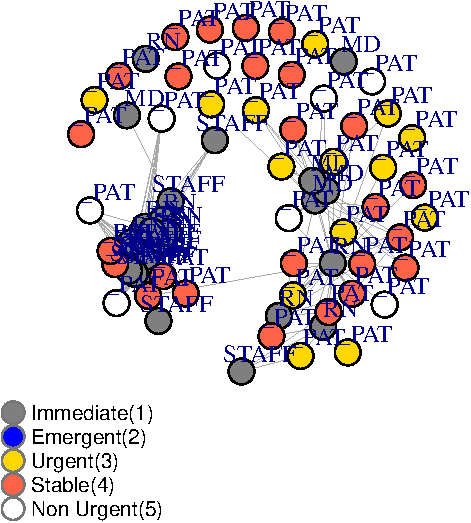
\includegraphics{Flynn_Project_files/figure-latex/shift 23-1.pdf} As I
am able to code more complex data and create better network graphs, and
analyze the structure of those graphs, this project will guide research
questions.
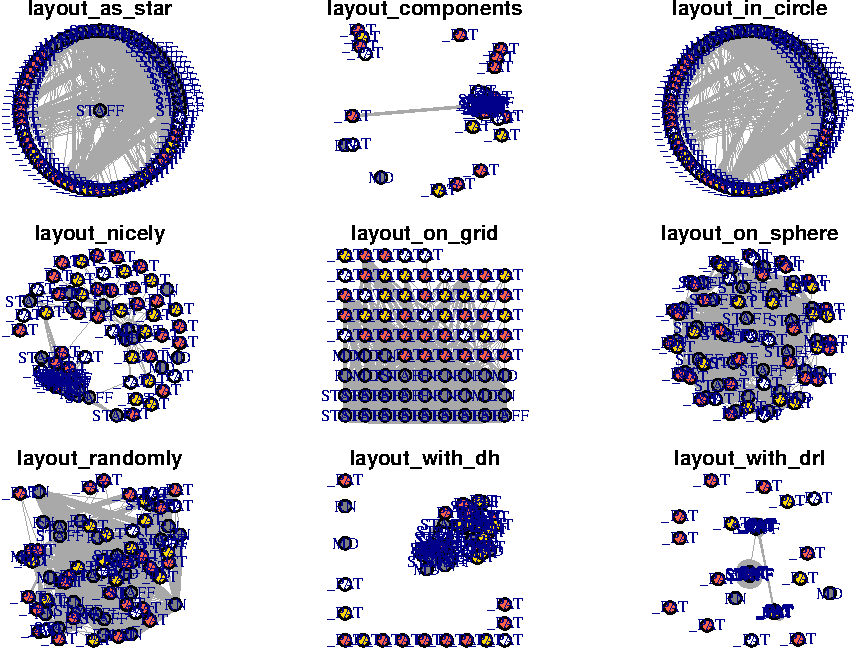
\includegraphics{Flynn_Project_files/figure-latex/shift23-1.pdf}
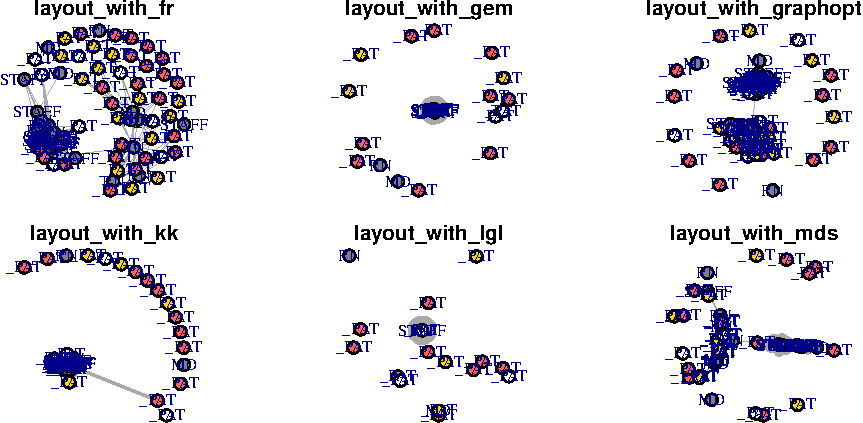
\includegraphics{Flynn_Project_files/figure-latex/shift23-2.pdf}

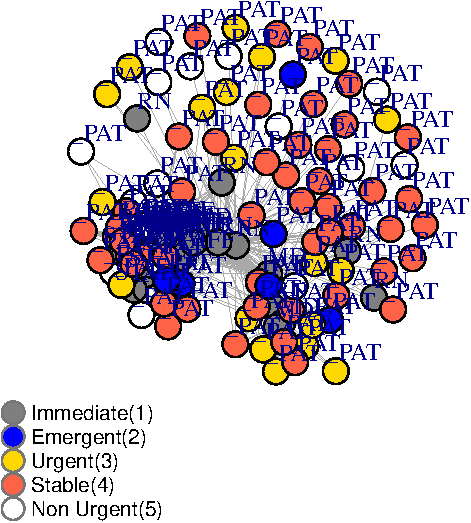
\includegraphics{Flynn_Project_files/figure-latex/shift13-1.pdf}

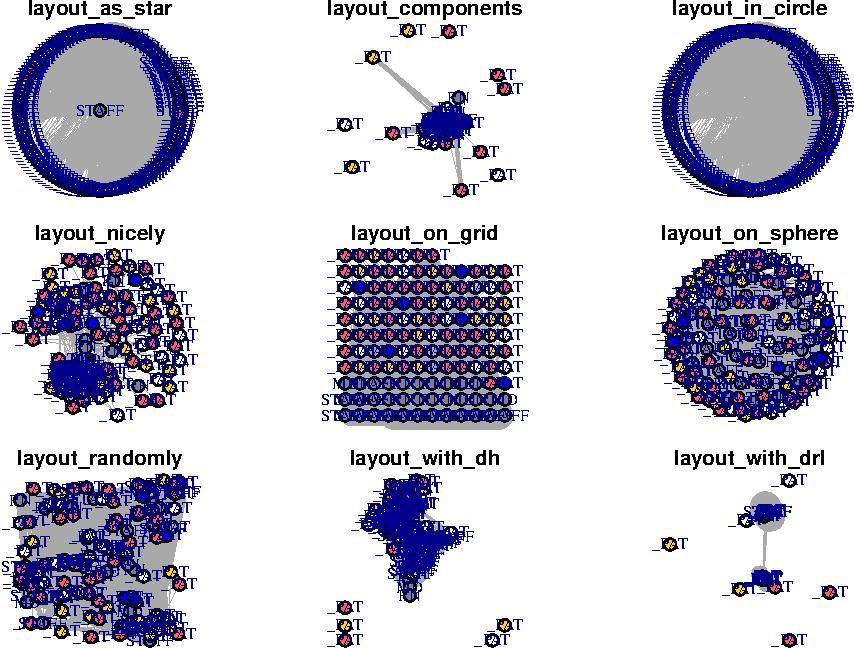
\includegraphics{Flynn_Project_files/figure-latex/unnamed-chunk-1-1.pdf}
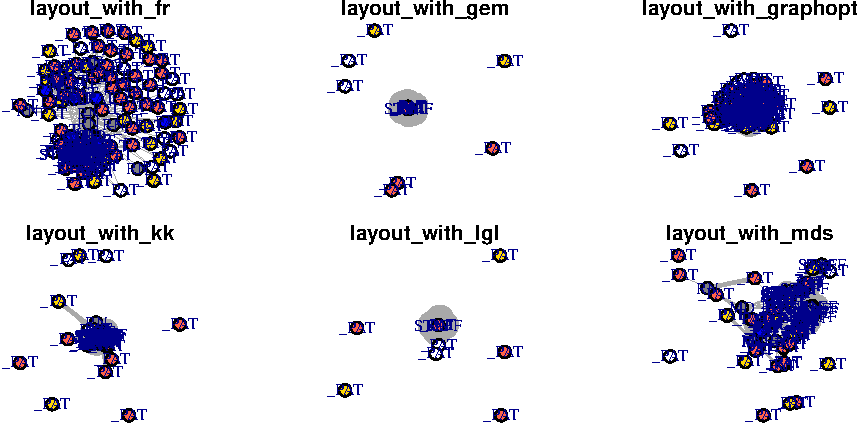
\includegraphics{Flynn_Project_files/figure-latex/unnamed-chunk-1-2.pdf}

\section{Discussion}\label{discussion}

Allocating staff resources in an Emergency Department is an ongoing
challenge. It also has important implications for patient safety and
health outcomes. The primary limitation to this study was the PI's lack
of experience with programming, the R programming language, and
statistical analysis. This project has been an important element in the
PI's learning process.

\section{Conclusion}\label{conclusion}

I was not able to finish my analysis and had to remove my second aim
which would have been interesting. However, as this is going to be the
analysis I do for my dissertation, the project is far from over. I look
forward to finding meaning in the real clinical interaction networks
that is reflected in the patterns and variations that is seen in the
graphs presented here.

\section*{References}\label{references.unnumbered}
\addcontentsline{toc}{section}{References}

\hypertarget{refs}{}
\hypertarget{ref-MARKDOWN}{}
Allaire, JJ, Jeffrey Horner, Vicent Marti, and Natacha Porte. 2017.
\emph{Markdown: 'Markdown' Rendering for R}.
\url{https://CRAN.R-project.org/package=markdown}.

\hypertarget{ref-RN602}{}
Canto, John G., Jeroan J. Allison, Catarina I. Kiefe, Contessa Fincher,
Robert Farmer, Padmini Sekar, Sharina Person, and Norman W. Weissman.
2000. ``Relation of Race and Sex to the Use of Reperfusion Therapy in
Medicare Beneficiaries with Acute Myocardial Infarction.'' Journal
Article. \emph{New England Journal of Medicine} 342 (15): 1094--1100.
doi:\href{https://doi.org/10.1056/NEJM200004133421505}{10.1056/NEJM200004133421505}.

\hypertarget{ref-IGRAPH}{}
Csardi, Gabor, and Tamas Nepusz. 2006. ``The Igraph Software Package for
Complex Network Research.'' \emph{InterJournal} Complex Systems: 1695.
\url{http://igraph.org}.

\hypertarget{ref-RN794}{}
Donoho, David. 2017. ``50 Years of Data Science.'' Journal Article.
\emph{Journal of Computational and Graphical Statistics} 26 (4):
745--66.
doi:\href{https://doi.org/10.1080/10618600.2017.1384734}{10.1080/10618600.2017.1384734}.

\hypertarget{ref-BEES}{}
Kridi, Douglas S., Carlos Giovanni N. de Carvalho, and Danielo G. Gomes.
2016. ``Application of Wireless Sensor Networks for Beehive Monitoring
and in-Hive Thermal Patterns Detection.'' \emph{Computers and
Electronics in Agriculture} 127: 221--35.
doi:\href{https://doi.org/https://doi.org/10.1016/j.compag.2016.05.013}{https://doi.org/10.1016/j.compag.2016.05.013}.

\hypertarget{ref-RN1X}{}
Lowery-North, Douglas W., Vicki Stover Hertzberg, Lisa Elon, George
Cotsonis, Sarah A. Hilton, II Vaughns Christopher F., Eric Hill, Alok
Shrestha, Alexandria Jo, and Nathan Adams. 2013. ``Measuring Social
Contacts in the Emergency Department.'' Journal Article. \emph{PLoS ONE}
8 (8): e70854.
doi:\href{https://doi.org/10.1371/journal.pone.0070854}{10.1371/journal.pone.0070854}.

\hypertarget{ref-CRAN}{}
R Core Team. 2017. \emph{R: A Language and Environment for Statistical
Computing}. Vienna, Austria: R Foundation for Statistical Computing.
\url{https://www.R-project.org/}.

\hypertarget{ref-RN251}{}
Tanabe, Paula, Rick Gimbel, Paul R. Yarnold, and James G. Adams. 2004.
``The Emergency Severity Index (Version 3) 5-Level Triage System Scores
Predict Ed Resource Consumption.'' Journal Article. \emph{Journal of
Emergency Nursing} 30 (1): 22--29.
doi:\href{https://doi.org/http://dx.doi.org/10.1016/j.jen.2003.11.004}{http://dx.doi.org/10.1016/j.jen.2003.11.004}.

\hypertarget{ref-GGPLOT2}{}
Wickham, Hadley. 2016. \emph{Ggplot2: Elegant Graphics for Data
Analysis}. Springer-Verlag New York. \url{http://ggplot2.org}.

\hypertarget{ref-TIDY}{}
---------. 2017. \emph{Tidyverse: Easily Install and Load the
'Tidyverse'}. \url{https://CRAN.R-project.org/package=tidyverse}.

\hypertarget{ref-RN257}{}
Yao, Wen, Chao-Hsien Chu, and Zang Li. 2012. ``The Adoption and
Implementation of Rfid Technologies in Healthcare: A Literature
Review.'' Journal Article. \emph{Journal of Medical Systems} 36 (6):
3507--25.
doi:\href{https://doi.org/10.1007/s10916-011-9789-8}{10.1007/s10916-011-9789-8}.

\hypertarget{ref-RN253}{}
Yu, Denny, Renaldo C. Blocker, Mustafa Y. Sir, M. Susan Hallbeck, Thomas
R. Hellmich, Tara Cohen, David M. Nestler, and Kalyan S. Pasupathy.
2015. ``Intelligent Emergency Department: Validation of Sociometers to
Study Workload.'' Journal Article. \emph{Journal of Medical Systems} 40
(3): 53.
doi:\href{https://doi.org/10.1007/s10916-015-0405-1}{10.1007/s10916-015-0405-1}.

\end{document}


